\chapter{Overview}
\label{atomics}


\begin{figure*}[!t]
	\centering
	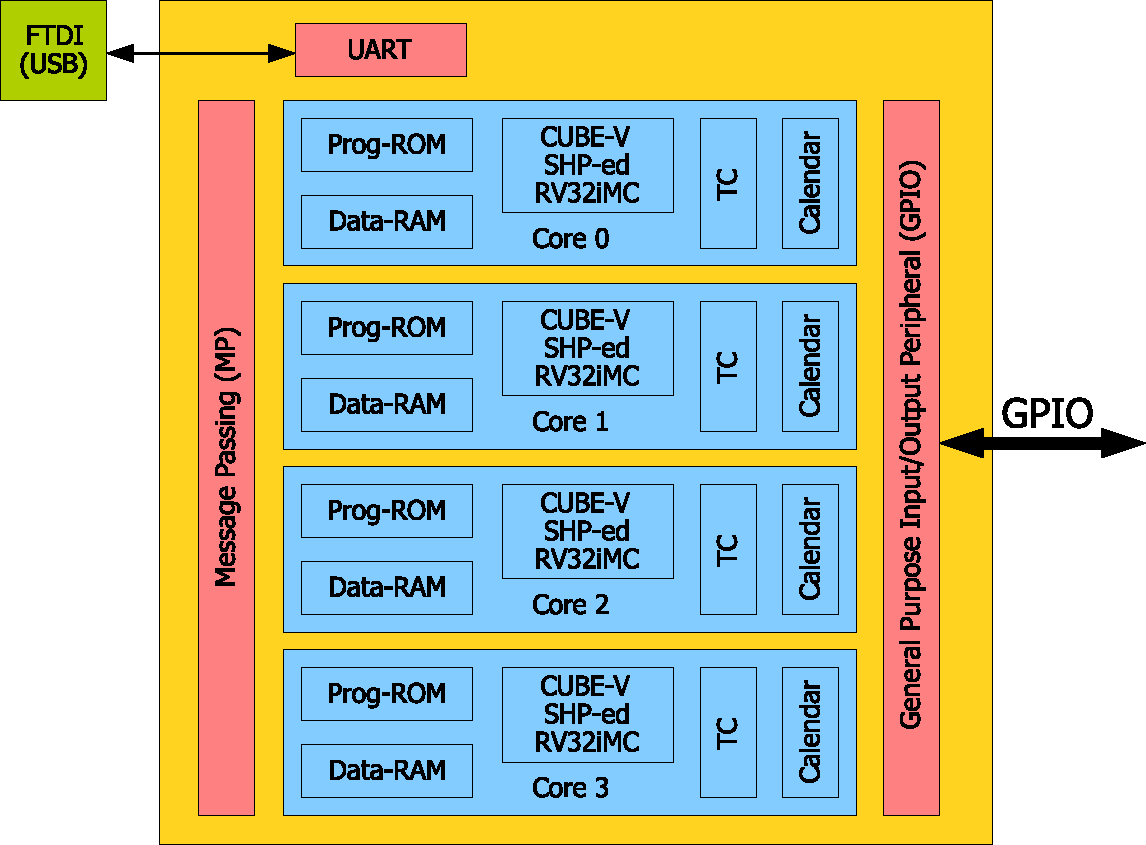
\includegraphics[width=4in]{figs/overview}
	\caption{Overview of the hardware.}
	\label{overview}
\end{figure*}


A cluster of a system hyper pipelined RV32iMC and its associated (program and data) memories as well as its thread controller and its calendar are considered as a subsystem which is called a ''core''. There are 4 cores implemented in the current version of the project. They can communicate with each other using message passing. They have equal rights to access the GPIO, yeah. Only core 0 can communicate with the UART, which is connected to the USB interface. An overview is given in Figure \ref{overview}.

